% The automaton of the multiples of 3 in binary (generated by figs_c3ch01.py).
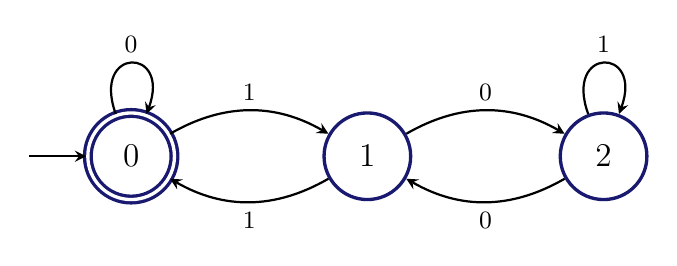
\begin{tikzpicture}[>=stealth,x=1cm,y=1cm,
  st/.style={circle,draw=MidnightBlue,very thick,minimum size=11mm,font=\large},
  lab/.style={font=\small,auto}]
\node[st,double,double distance=1.2pt] (q0) at (0,0) {$0$};
\node[st] (q1) at (3,0) {$1$};
\node[st] (q2) at (6,0) {$2$};
\draw[->,thick] (-1.3,0) -- (q0);
\draw[->,thick] (q0) to[bend left=30] node[lab] {$1$} (q1);
\draw[->,thick] (q1) to[bend left=30] node[lab] {$1$} (q0);
\draw[->,thick] (q1) to[bend left=30] node[lab] {$0$} (q2);
\draw[->,thick] (q2) to[bend left=30] node[lab] {$0$} (q1);
\draw[->,thick] (q0) to[out=110,in=70,looseness=6] node[lab] {$0$} (q0);
\draw[->,thick] (q2) to[out=110,in=70,looseness=6] node[lab] {$1$} (q2);
\end{tikzpicture}
